

\section{2.幺正变换}

\begin{frame}
    \frametitle{前情回顾}
    \begin{itemize}
       \done 波函数,力学量算符,公式在Q表象下的矩阵表示 
       \todo 表象变换
    \end{itemize}
\end{frame} 

\subsection{幺正变换的定义}

\begin{frame} 
    \frametitle{}
    \begin{tcolorbox1}{幺正矩阵和厄密矩阵}
        \begin{enumerate}
            \Item F的逆算符$F^{-1}F=FF^{-1}=I$, $$F\Psi=\psi, \qquad \Psi=F^{-1}\psi$$  
            \Item F的共轭算符(称伴算符) $F^{\dagger}=(F_{nm} ^*)^T$, $$ (\psi, F\Psi), \qquad (F^{\dagger}\psi, \Psi)$$
            如果$F^{\dagger } =F$,称F为{\color{red}厄密算符(矩阵)}, 
            判定: $F_{mn}=F_{nm} ^*$; 
            \\ 如果$ F^{\dagger }=F^{-1}$,称F为{\color{red} 幺正算符(矩阵)}, 判定:$F^{\dagger} F= FF^{\dagger}=I$
        \end{enumerate}       
    \end{tcolorbox1}
\end{frame}

\begin{frame} 
    \frametitle{}
    \begin{tcolorbox1}{幺正变换的定义}
    通过幺正矩阵联系起来的两矩阵之间的变换,称为幺正变换。
    \end{tcolorbox1}
\end{frame}

\begin{frame}     
    \例[1. 试证明二维平面矢量绕原点的旋转变换是幺正变换]{}
    \begin{wrapfigure} {r} {0.30\textwidth} %;图在右
        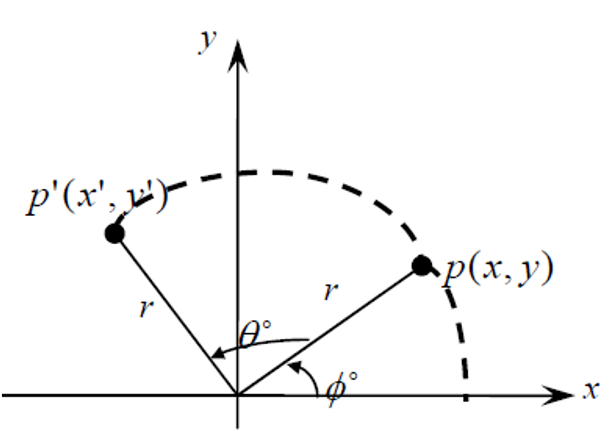
\includegraphics[width=0.29\textwidth]{figs/transf1.png}   
    \end{wrapfigure}
    \证~
    $\left\{\begin{matrix}
        x'=x\cos\theta -y\sin\theta\\
        y'=x\sin\theta+y\cos\theta
    \end{matrix}\right.$ \quad
    $\begin{bmatrix}
        x' \\
        y'
    \end{bmatrix}
    =
    \begin{bmatrix}
        \cos\theta & -\sin\theta\\
        \sin\theta & \cos\theta
    \end{bmatrix}
    \begin{bmatrix}
        x \\
        y
    \end{bmatrix}$\\
    $$ R_\theta=
    \begin{bmatrix}
        \cos\theta &-\sin\theta\\
        \sin\theta &\cos\theta
    \end{bmatrix} ,\qquad
    R_\theta ^{\dagger}=
    \begin{bmatrix}
        \cos\theta &\sin\theta\\
        -\sin\theta &\cos\theta
    \end{bmatrix} $$
    $$ R_\theta  R_\theta ^{\dagger} = R_\theta ^{\dagger} R_\theta=  
    \begin{bmatrix}
        \cos\theta &-\sin\theta\\
        \sin\theta &\cos\theta
    \end{bmatrix}
    \begin{bmatrix}
        \cos\theta &\sin\theta\\
        -\sin\theta &\cos\theta
    \end{bmatrix}
    =I
    $$
    证毕!
\end{frame}

\subsection{量子力学中的三种基本变换}

\begin{frame} 
    \frametitle{基矢变换}
    \例[2.试证明量子力学不同表象基组之间的变换是幺正变换]{}  
    \证~ 设A的基组为$\psi_\alpha$ B的基组为 $\varphi_n$, A归一化公式中把波函数在B展开: 
    \begin{equation*}
        \begin{split}
            \delta_{\alpha\beta} &= (\psi_\alpha, \psi_\beta) \\
            &= (\sum_n S_{n\alpha} \varphi_n, \sum_m S_{m\beta} \varphi_m)\\
            &= \sum_{nm} S_{n\alpha} ^* S_{m\beta}(\varphi_n, \varphi_m)\\
            &= \sum_{nm} S_{n\alpha} ^* S_{m\beta}\delta_{nm}\\
            &= \sum_{n} S_{n\alpha} ^* S_{n\beta} = \sum_{n} S^{\dagger } _{\alpha n} S_{n\beta}
        \end{split} 
    \end{equation*}
\end{frame}

\begin{frame} 
    B归一化公式也可在A展开: 
    \begin{equation*}
        \begin{split}
            \sum_{\alpha} S_{n\alpha}  S^{\dagger } _{\alpha m}&=\sum_{\alpha} S_{n\alpha}  S_{m \alpha} ^* \\
            &=\sum_{\alpha} (\varphi_n, \psi_\alpha) (\varphi_m, \psi_\alpha)^* \\
            &=\sum_{\alpha} (\psi_\alpha,\varphi_n)^* (\psi_\alpha,\varphi_m) \\
            &=\sum_{\alpha\beta} (\psi_\alpha,\varphi_n)^* (\psi_\beta,\varphi_m) \delta_{\alpha\beta} \\
            &=\sum_{\alpha\beta} S_{\alpha n}^*  S_{\beta m} (\psi_\alpha,\psi_\beta)\\
            &= (\sum_{\alpha} S_{\alpha n}\psi_\alpha,\sum_{\beta} S_{\beta m}\psi_\beta)\\
            &= (\varphi_n,\varphi_m) =\delta_{nm} 
        \end{split} 
    \end{equation*}
\end{frame}

\begin{frame} 
    因此,我们有:
    \begin{equation*}
        \begin{split}
            \sum_{\alpha} S_{n\alpha}   S^{\dagger } _{\alpha m} &=\delta_{nm} \\
            \sum_{n} S^{\dagger } _{\alpha n} S_{n\beta}&=\delta_{\alpha\beta}
        \end{split} 
    \end{equation*}
    即:$$ S^{\dagger }S=SS^{\dagger } =I$$ 
    证毕! \\

    注意到: $ S_{n\alpha} = (e_n, e_\alpha)= (e_{(B)}, e_{(A)})$ \\
    得变换公式: $$ \color{red} u_{(B)}= S^{\dagger} u_ {(A)}$$
\end{frame}


\begin{frame} {波函数变换}
    \例[3.试证明同一波函数在两不同表象中的矩阵之间的变换是幺正变换]{}  
    \证~ 设A的基组为$\psi_\alpha$ B的基组为 $\varphi_n$\\
    波函数$\Psi$在A表象和B表象中分别展开:
    \begin{equation*}
        \begin{split}
            \sum_\alpha a_\alpha \psi_\alpha &= \sum_n b_n \varphi_n \\
            \sum_\alpha a_\alpha \psi_\beta ^* \psi_\alpha &= \sum_n b_n \psi_\beta ^* \varphi_n \\
            \sum_\alpha a_\alpha (\psi_\beta, \psi_\alpha) &= \sum_n b_n (\psi_\beta, \varphi_n) \\
            \sum_\alpha a_\alpha \delta_{\alpha\beta} &= \sum_n b_n (\psi_\beta, \varphi_n) \\
            a_\alpha &= \sum_n S_{\alpha n} b_n\\
        \end{split} 
    \end{equation*}
\end{frame}

\begin{frame} 
    \begin{equation*}
        \begin{split}
            \Psi &= \\
            a_\alpha &= \sum_n S_{\alpha n} b_n\\
            a&=Sb\\
            \color{red} b& \color{red}=S^{\dagger}a   
        \end{split} 
    \end{equation*}
    正是两基组之间的幺正矩阵\\
    证毕!\\
\end{frame}


\begin{frame} {算符变换}
    \例[4.试证明同一力学量算符在两不同表象中的矩阵变换是幺正变换]{}  
    \证~ 设A的基组为$\psi_\alpha$ B的基组为 $\varphi_n$\\
    算符F在A表象的矩阵元为$F_{\alpha\beta}$, 在B表象中的矩阵元为$F'_{nm}$
    \begin{equation*}
        \begin{split}
            F'_{nm} &= (\varphi_n, F\varphi_m) \\
            &= (\sum_{\alpha} S_{\alpha n}\psi_\alpha, F \sum_{\beta} S_{\beta m}\psi_\beta)\\
            &= \sum_{\alpha\beta} S_{\alpha n} ^* (\psi_\alpha, F \psi_\beta) S_{\beta m}\\
            &= \sum_{\alpha\beta} S_{\alpha n} ^* F_{\alpha\beta} S_{\beta m}
        \end{split} 
    \end{equation*}
\end{frame}


\begin{frame} 
    \begin{equation*}
    \begin{split}
        F'_{nm} &= \sum_{\alpha\beta} S_{n\alpha } ^{\dagger} F_{\alpha\beta} S_{\beta m} \\
        &= (S^{\dagger} F S)_{nm}
    \end{split} 
    \end{equation*} 
    $$\color{red} F'= S^{\dagger} F S $$
\end{frame}

\subsection{幺正变换的性质}

\begin{frame} {幺正变换性质1:}
    \例[5.试证明幺正变换不改变算符的本征值]{} 
    \证~算符F在A表象的矩阵为F,本征矢为a, 在B表象中的矩阵为F' 本征矢为b,有本征方程:
    \begin{equation*}
        \begin{split}
            Fa&=fa \qquad (1)\\
            F'b&=f'b\\
            S^{\dagger} F S S^{\dagger}a &=f'S^{\dagger}a\\
            S^{\dagger} F a &=f'S^{\dagger}a\\
            SS^{\dagger} F a &=f'SS^{\dagger}a\\
            F a &=f'a \qquad (2)\\
        \end{split} 
    \end{equation*} 
    比较(1)(2)式,有$f=f'$, 证毕!
\end{frame}    

\begin{frame} {幺正变换性质2:}
    \例[6.试证明幺正变换不改变矩阵的迹]{}
    \证 ~矩阵A的对角元素之和称为矩阵A的迹,用$SP(A)$或$tr(A)$表示,则性质\\
    $$tr(AB)=tr(BA) $$
    \begin{equation*}
        \begin{split}
            tr(AB) &=\sum_i (AB)_{ii}\\
            &=\sum_{i} \sum_{j} (A_{ij} B_{ji}) \\
            &=\sum_{i} \sum_{j} (B_{ji} A_{ij}) \\
        \end{split} 
    \end{equation*} 
\end{frame}    


\begin{frame}     
    \begin{equation*}
        \begin{split}
            tr(AB) &=\sum_{j} \sum_{i} (B_{ji} A_{ij}) \\
            &=\sum_{j} (BA)_{jj} \\
            &=tr(BA)
        \end{split} 
    \end{equation*}

    \begin{equation*}
        \begin{split}
            F'&= S^{\dagger} F S \\
            tr(F')&=tr(S^{\dagger} F S)\\
            &=tr(SS^{\dagger}  F)\\
            &=tr(F)\\
        \end{split} 
    \end{equation*} 
    证毕!
\end{frame}    

\begin{frame} {幺正变换性质3:}
    \例[7.幺正变换不改变物理规律,现已知在 x 表象中的基本对易关系$xp_x-p_x x =i\hbar$, 试求它在p表象中的形式,然后证明这种对易关系不随表象发生变化]{}
    \解 ~(1)在p表象, $$ \hat{x}=i\hbar\dfrac{\partial}{\partial p_x}, \qquad \hat{p}_x=p_x $$
     对任意波函数 $\Psi(p_x)$
    \begin{equation*}
        \begin{split}
            \hat{x}\hat{p}_x\Psi &= i\hbar\dfrac{\partial}{\partial p_x} (p_x \Psi )\\
            &= i\hbar\Psi + p_xi\hbar\dfrac{\partial}{\partial p_x}\Psi \qquad (a)\\
        \end{split} 
    \end{equation*} 

\end{frame}  
\begin{frame} 
    $$\hat{p}_x\hat{x}\Psi = p_x(i\hbar\dfrac{\partial}{\partial p_x}\Psi) \qquad (b)$$
    (a)-(b)
    $$\hat{x}\hat{p}_x\Psi-\hat{p}_x\hat{x}\Psi=i\hbar\Psi$$
    $$\hat{x}\hat{p}_x-\hat{p}_x\hat{x}=i\hbar$$
    (2) 在Q表象,$$ x'= S^\dagger x S, \qquad p'_x= S^\dagger p_x S $$
    \begin{equation*}
        \begin{split}
        x'p'_x-p'_x x' &= S^\dagger x S S^\dagger p_x S - S^\dagger p_x S S^\dagger x S \\
        &= S^\dagger x p_x S - S^\dagger p_x x S \\
        &= S^\dagger (x p_x -  p_x x) S \\
        &= i\hbar S^\dagger S \\
        &= i\hbar \\
        \end{split} 
    \end{equation*} 
\end{frame}  
\begin{frame}
    \begin{tcolorbox2}{推论:}
       \begin{enumerate}
           \Item 量子体系进行任一幺正变换不改变它的全部物理内容
           \Item 两个量子体系,如果能用幺正变换联系起来,则它们在物理上是等价的
       \end{enumerate} 
    \end{tcolorbox2}
\end{frame}

\begin{frame}{构造S矩阵的方法}
        \例[8.已知算符F在A表象中的矩阵如下,求F表象和A表象之间的幺正变换矩阵S]
        {$$ H=
        \begin{bmatrix}
            2\varepsilon  & 0 & \varepsilon\\
            0 & 2\varepsilon & 0 \\
            \varepsilon & 0 & 2\varepsilon\\
        \end{bmatrix} $$}
     \解~ 如果知道A表象的基 $\{\psi_\alpha \}$, F表象的基 $ \{\varphi_n \}$, 则可直接通过计算内积得到:
     $$ S_{n\alpha} =(\varphi_n, \psi_\alpha) $$
     现在知道一个非对角矩阵H,我们可以通过解久期方程得到本征值和本征函数,得到一个对角阵H',这相当于实现了一个从A表象到H表象的幺正变换,关系式为:
     $$ H'=S^\dagger H S$$
\end{frame}  

\begin{frame}
    \例[9.试证明F在A表象的本征函数系构成这个S矩阵]{}
    \证~ 注意到H'的对角元是本征值
    \begin{equation*}
    \begin{split}
    H' &=S^\dagger H S \\
    H'_{mn} &=(S^\dagger H S)_{mn}  \\
    \sum_{\alpha \beta} S^{\dagger} _{m \alpha} H_{\alpha \beta} S_{\beta n} & = h_m \delta_{mn} \\
    \sum_{\alpha \beta} (\sum_m S_{\alpha m} S^\dagger_{m \alpha}) H_{\alpha \beta} S_{\beta n} &= h_m \sum_m S_{\alpha m}\delta_{mn} \\
    \sum_{\beta} H_{\alpha \beta} S_{\beta n} &= h_n S_{\alpha n} \\
    \end{split} 
    \end{equation*} 
    上式表明,第n个本征态正好是S矩阵的第n列!\\
    即依次提列本征函数构成S阵。证毕!
\end{frame} 

%%%%%%%%%%%%%%%%%%%%%%%%%%%%%%%%%%%%%%%%%%%%%%%%%%%%%%%%%%%%%%%%%%%
\begin{frame}
    \frametitle{课外作业}
    \begin{enumerate}
        \item 算符F在A表象的矩阵如下(其中$\theta$为实常数) \\ 
        \[ F= \begin{pmatrix}
          0 & e^{\theta} \\
          e^{-\theta} & 0 \\
        \end{pmatrix} \]
        (1)求F的本征值和正交归一本征矢在A表象的具体表示\\
        (2)求使F对角化的幺正变换矩阵S
        \item 已知两可观测力学量算符A,B. 满足 $A^2=B^2=I, \quad AB+BA=0$,求 \\ 
              (1) 算符A,B的本征值 \\ 
              (2) 在A表象中A,B及它们的本征矢的具体表示 \\ 
              (3) 在B表象中A,B及它们的本征矢的具体表示 \\ 
              (4) 从A到B的幺正变换矩阵S
    \end{enumerate}
\end{frame}
%%%%%%%%%%%%%%%%%%%%%%%%%%%%%%%%%%%%%%%%%%%%%%%%%%%%%%%%%%%%%%%%%%%

 

